\documentclass{beamer}
\usetheme{Madrid}
\usepackage{graphicx}
\graphicspath{{figs/}}

\title{Steering vs.\ Scaffolding in LatentMAS}
\subtitle{Can we steer the latent handoff --- and do the latent agents earn their keep?}
\author{Sagnik Biswas}
\date{July 2026}

\begin{document}

\begin{frame}
    \titlepage
    \vspace{-1cm}
\end{frame}

\begin{frame}{Where We Were}
    \textbf{Prior finding:} SEAL steering of the \textbf{Judger} cuts output tokens $\sim$25--39\% at held accuracy; steering the \emph{latent} agents did nothing to tokens.
    \vspace{0.3cm}
    \begin{itemize}
        \item Leverage sat at the \textbf{text-emitting Judger}, not the latent agents.
        \item Two follow-up questions this raised:
    \end{itemize}
    \vspace{0.2cm}
    \begin{block}{This deck: two experiments}
        \textbf{1. KV Cache Steering.} The latent agents only speak through the KV cache they hand the Judger. Can we steer \emph{that handoff} to make them useful?
        \\[0.2cm]
        \textbf{2. Agent Ablation.} Simpler question first --- do Planner/Critic/Refiner improve the system \emph{at all}, or is the Judger doing the work?
    \end{block}
\end{frame}

\begin{frame}{Recap: LatentMAS in One Slide}
    \begin{center}
        [Question] $\rightarrow$ Planner $\rightarrow$ Critic $\rightarrow$ Refiner $\rightarrow$ \textbf{Judger} $\rightarrow$ [Answer]
    \end{center}
    \vspace{0.3cm}
    \begin{itemize}
        \item Planner/Critic/Refiner run \textbf{40 latent steps} each, emit \textbf{no text}.
        \item They grow a shared \textbf{KV cache} --- the entire inter-agent ``message.''
        \item Only the \textbf{Judger} decodes text $\Rightarrow$ the sole source of output tokens.
    \end{itemize}
    \vspace{0.3cm}
    \begin{center}\textit{The handoff is a memory channel, not a text channel.}\end{center}
\end{frame}

% ---------------- Experiment 1: KV cache steering ----------------
\begin{frame}{Experiment 1: KV Cache Steering (arXiv:2507.08799)}
    \textbf{Idea:} one-shot edit of the cache the Judger reads, then decode normally.
    \vspace{0.2cm}
    \begin{itemize}
        \item Direction $S$ from \textbf{CoT-rich vs.\ answer-only} prompt pairs (mean-of-differences on final-token K/V), value-only ($c_k=0$).
        \item Apply once, all layers: $\;V \mathrel{+}= c_v\, S_v\;$ at chosen cache positions.
        \item \textbf{Surfaces tested:} the latent \textbf{handoff} (last col / all cols) vs.\ the \textbf{Judger's own} final prompt token (paper's target, as a control).
    \end{itemize}
    \vspace{0.2cm}
    \begin{center}\textit{Unlike SEAL (per-step residual hook), this is one-shot and zero added latency.}\end{center}
\end{frame}

\begin{frame}{Experiment 1: Results (GSM8K, n=150)}
    \textbf{Control (star): 94.7\% acc, 588 Judger tokens}
    \begin{center}
        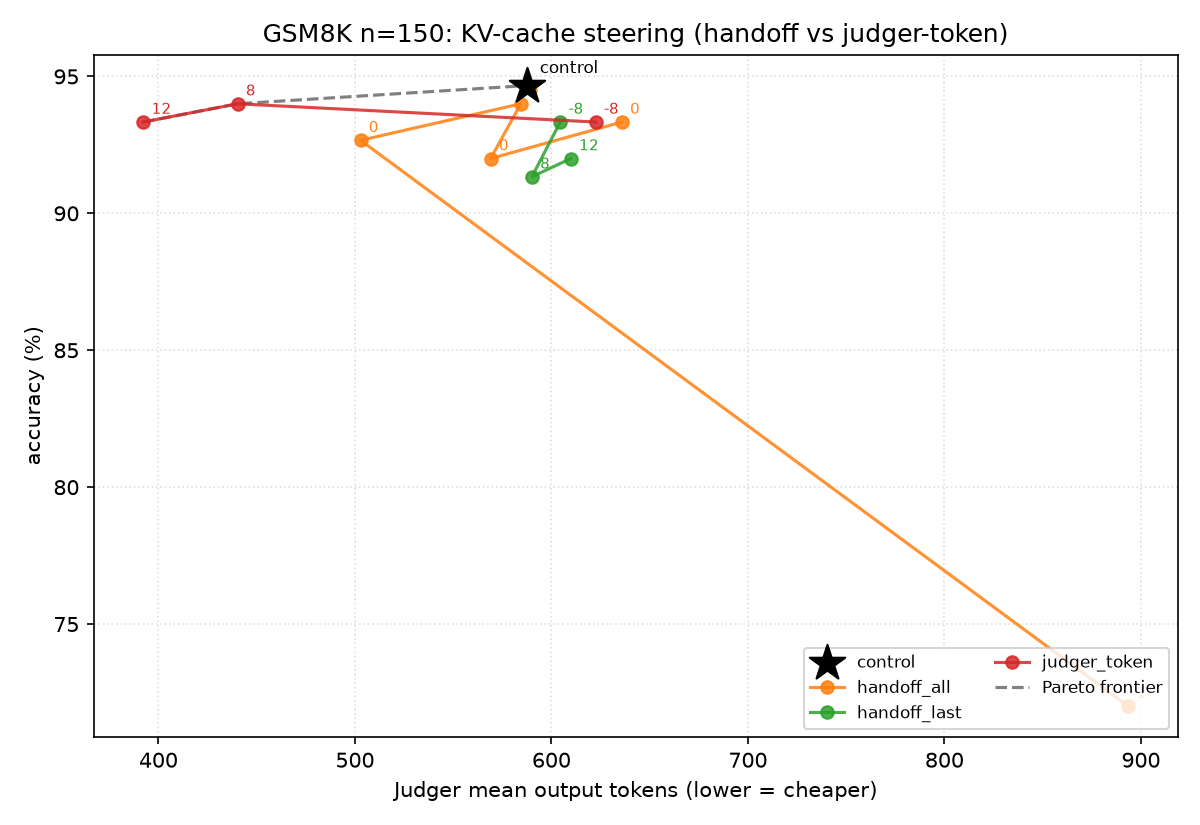
\includegraphics[width=0.72\textwidth]{kv_gsm8k.png}
    \end{center}
    \vspace{-0.2cm}
    \begin{itemize}
        \item \textbf{Handoff} steering (orange/green) = no gain; $c_v{=}1$ crashes to 72\% / 894 tok.
        \item \textbf{Judger token} (red) = the frontier: $-25\%$ ($c_v{=}8$) to $-33\%$ ($c_v{=}12$) tokens, accuracy held.
    \end{itemize}
\end{frame}

\begin{frame}{Experiment 1: Why the Handoff Resists Steering}
    \textbf{Attention weights sum to 1.}
    \begin{itemize}
        \item Steering \emph{all} handoff columns shifts the Judger's attention output by the \textbf{full} $c_v S_v$ every layer $\Rightarrow$ saturates into oversteering almost immediately ($c_v{=}1$ collapses 94.7\%$\rightarrow$72\%).
        \item Steering \emph{one} column $=$ $\sim$1/130 of attention $\Rightarrow$ too weak to matter.
    \end{itemize}
    \vspace{0.3cm}
    \begin{block}{Takeaway}
        The KV cache has two position types: \textbf{dense information} positions (latent thoughts) that steering \emph{corrupts}, and \textbf{aggregation} positions (last prompt token) that steering \emph{rides}. Cache steering works --- but only on the Judger's own context.
    \end{block}
\end{frame}

% ---------------- Experiment 2: ablation ----------------
\begin{frame}{Experiment 2: Do the Latent Agents Earn Their Keep?}
    \textbf{Two negatives (residual SEAL, KV steering) $\Rightarrow$ ask the base question.}
    \vspace{0.2cm}
    \begin{itemize}
        \item \textbf{Ablate the chain} and measure accuracy, tokens, latency, compute:
        \begin{center}
            judger\_only $\rightarrow$ +Planner $\rightarrow$ +Critic $\rightarrow$ full
        \end{center}
        \item Prefix chain $=$ marginal value of each added agent (every agent's prompt still gets the upstream context it expects).
        \item \textbf{Key design point:} GSM8K is near-ceiling ($\sim$93\%) for Qwen3-14B $\Rightarrow$ underpowered for accuracy. Run the accuracy question on \textbf{MedQA} (headroom, $\sim$74\%).
    \end{itemize}
\end{frame}

\begin{frame}{Experiment 2: GSM8K (n=300) --- Efficiency, Not Accuracy}
    \begin{center}
        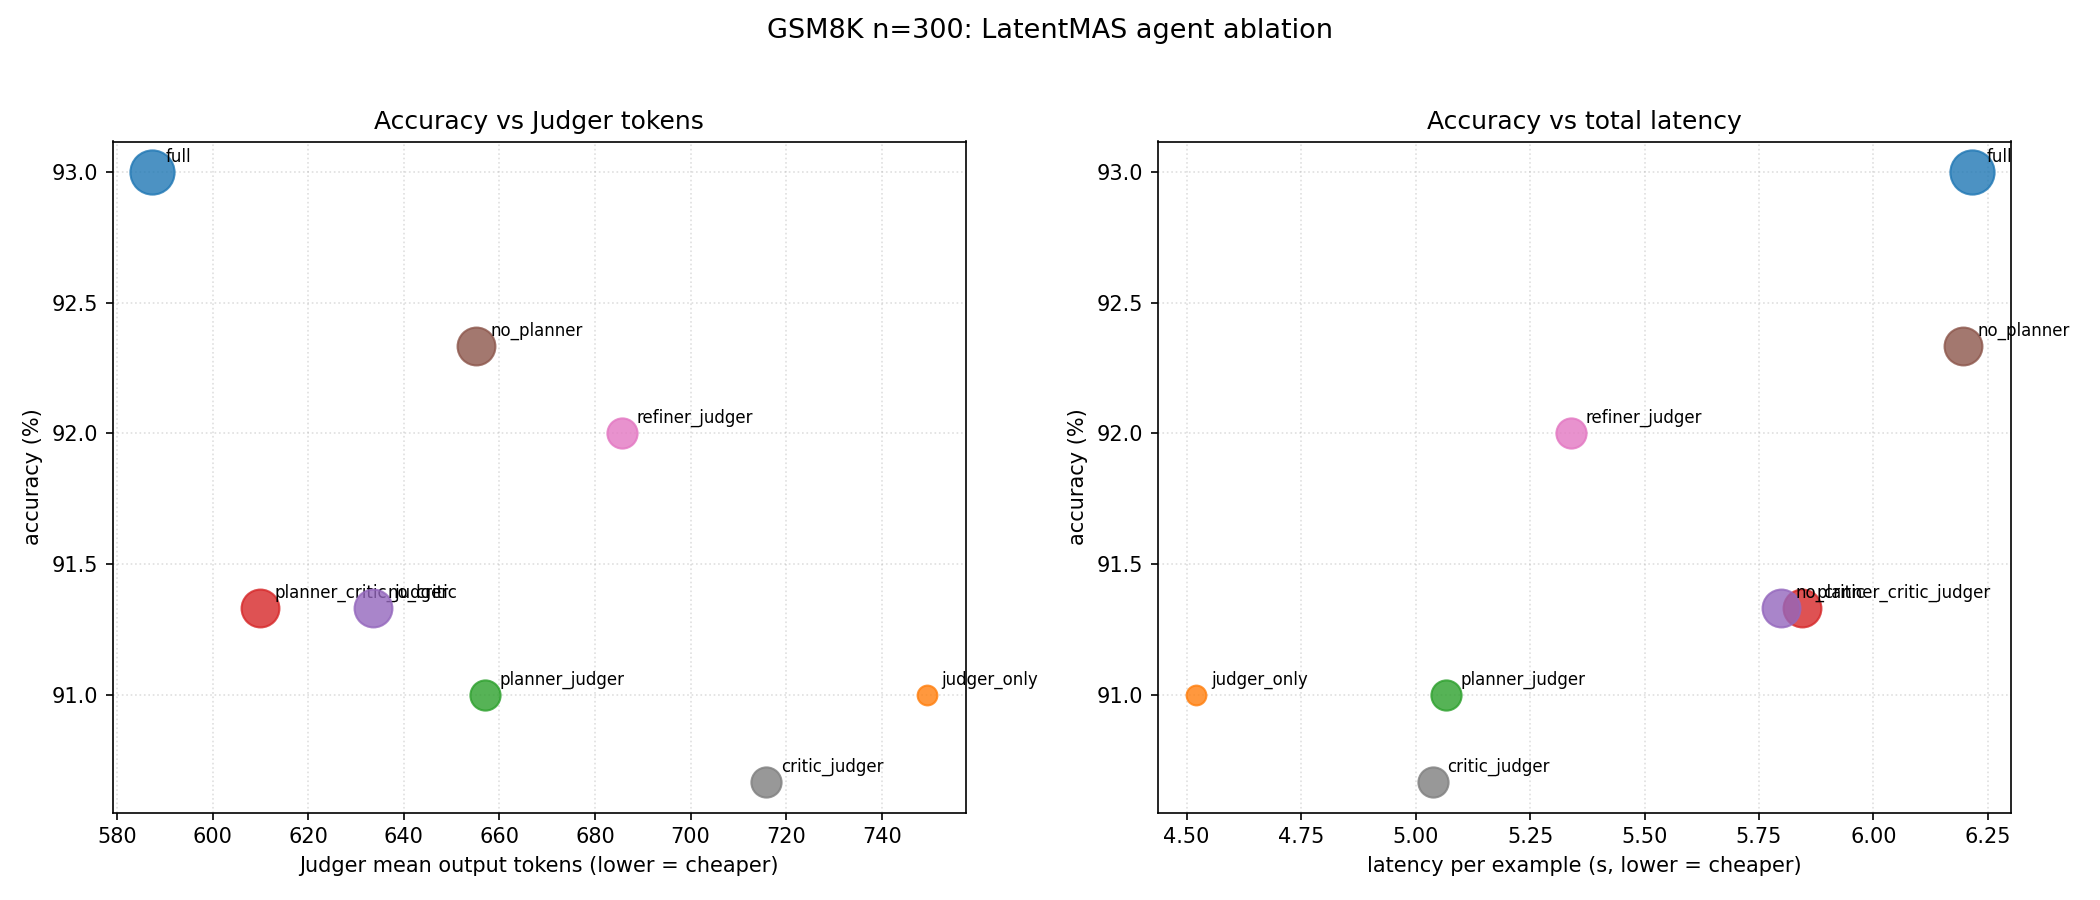
\includegraphics[width=0.98\textwidth]{ablation_gsm8k.png}
    \end{center}
    \vspace{-0.2cm}
    \begin{itemize}
        \item Accuracy \textbf{flat} (91$\rightarrow$93\%, within noise --- ceiling); tokens fall \textbf{monotonically} with scaffold depth ($749\rightarrow587$, $-22\%$) but latency rises.
        \item $\Rightarrow$ on an easy task, the agents are a \textbf{conciseness} knob, not an accuracy one.
    \end{itemize}
\end{frame}

\begin{frame}{Experiment 2: MedQA (n=300, 2 seeds) --- The Reversal}
    \textbf{On the task with headroom, the scaffold \emph{hurts}.}
    \vspace{0.2cm}
    \begin{table}[]
        \centering\small
        \begin{tabular}{|l|c|c|c|}
            \hline
            \textbf{Config} & \textbf{Acc (s42/s123)} & \textbf{Tokens} & \textbf{s/ex} \\ \hline
            \textbf{judger\_only} & \textbf{73.7 / 75.0} & \textbf{$\sim$885} & \textbf{5.7} \\ \hline
            planner\_judger & 71.3 / 68.7 & $\sim$1130 & 7.6 \\ \hline
            planner\_critic\_judger & 70.3 / 69.0 & $\sim$1020 & 9.7 \\ \hline
            full & 71.7 / --- & $\sim$997 & 11.7 \\ \hline
        \end{tabular}
    \end{table}
    \vspace{0.2cm}
    \begin{itemize}
        \item \textbf{judger\_only is best} --- adding agents \emph{lowers} accuracy (both seeds).
        \item Upstream agents \emph{raise} tokens and \textbf{double latency} ($\sim$2$\times$).
    \end{itemize}
\end{frame}

\begin{frame}{Conclusion}
    \begin{center}
        \Large \textbf{Core Message} \\
        \vspace{0.5cm}
        \normalsize
        Steering the latent \textbf{handoff} does not help --- the dense KV channel is not a linear steering surface. And on a task with headroom (MedQA), the \textbf{latent scaffold actively degrades} accuracy while roughly \textbf{doubling compute}.
        \\[0.4cm]
        \textbf{Leverage lives at the text-emitting Judger.} A single well-steered Judger beats the 4-agent scaffold here --- on accuracy, tokens, \emph{and} latency.
    \end{center}
\end{frame}

\begin{frame}{Limitations \& Next Steps}
    \textbf{Limitations}
    \begin{itemize}
        \item n=150--300, 1--2 seeds; single backbone (Qwen3-14B); MedQA capped at 300 items.
        \item KV vector from text CoT applied to latent KV (modality gap); $c_k=0$ only.
        \item Default fork runs realignment $W_a$ off --- worth a faithfulness re-check.
    \end{itemize}
    \vspace{0.2cm}
    \textbf{Next steps}
    \begin{itemize}
        \item Confirm the MedQA reversal on GPQA / a second hard task.
        \item Head-to-head: one-shot \textbf{judger-token cache steering} vs.\ per-step SEAL hook (accuracy, tokens, latency).
        \item If the scaffold doesn't pay: \textbf{simplify to a single steered Judger}.
    \end{itemize}
\end{frame}

\end{document}
